\documentclass[12pt,letterpaper]{article}

\usepackage[utf8]{inputenc}
\usepackage[T1]{fontenc}
\usepackage[english]{babel}
\usepackage{amsmath, amssymb, amsthm}
\usepackage{float, enumitem, xcolor, geometry}
\usepackage{graphicx, fancyhdr, fancyvrb}
\usepackage{array, makecell}
\usepackage{forest}
\usepackage[normalem]{ulem}
\usepackage[colorlinks=true, linkcolor=linkblue, urlcolor=linkblue, citecolor=linkblue]{hyperref}
\usepackage{makecell}
\usepackage{tikz}
\usepackage{svg}
\usetikzlibrary{automata, positioning, arrows.meta}

\definecolor{linkblue}{HTML}{1A167A}

\geometry{margin=2cm, top=2cm, bottom=2cm}

\newcommand{\pred}{$\rightarrow$}
\newcommand{\asig}{$\leftarrow$}

\newcommand{\nt}[1]{\textit{#1}}
\newcommand{\tk}[1]{\texttt{#1}}
\newcommand{\First}[1]{\mathrm{FIRST}(#1)}
\newcommand{\eps}{\varepsilon}

% ========================================
% COLORES
% ========================================
\definecolor{green_checkmark}{HTML}{07E314}
\definecolor{red_cross}{HTML}{ED4728}

% ========================================
% COMANDOS PARA MARCADORES
% ========================================
\newcommand{\greencheck}{\textcolor{green_checkmark}{$\checkmark$}}
\newcommand{\redcross}{\textcolor{red_cross}{$\times$}}

% ========================================
% CONSTANTES DEL ENCABEZADO
% ========================================
\newcommand{\encabezadoIzq}{Compiladores 2027-1}
\newcommand{\encabezadoCen}{Tarea 2}
\newcommand{\encabezadoDer}{\textit{Minim, deriv, elim y EBNF}}

% ========================================
% CONFIGURACION DEL ENCABEZADO
% ========================================
\pagestyle{fancy}
\fancyhf{}

\fancyhead[L]{\encabezadoIzq}
\fancyhead[C]{\encabezadoCen}
\fancyhead[R]{\encabezadoDer}

\fancyfoot[C]{\thepage}

\renewcommand{\headrulewidth}{0.1pt}
\renewcommand{\footrulewidth}{0pt}

% ========================================
% CONFIGURACION DE TABLAS
% ========================================
\newcolumntype{C}[1]{>{\centering\arraybackslash}m{#1}}
\newcolumntype{L}[1]{>{\raggedright\arraybackslash}m{#1}}
\newcolumntype{R}[1]{>{\raggedleft\arraybackslash}m{#1}}

\begin{document}

\thispagestyle{empty}
\begin{titlepage}
  \thispagestyle{empty}
  %--------------- COMANDO LINEA----------------->
  \newcommand{\linea}{\rule{\linewidth}{0.5mm}}                 
  \center
  %<<<<<<<<<<<<<<<<<<<<<<<<<<<<<<<<<<<<<<<<<<<

  %Add logos
  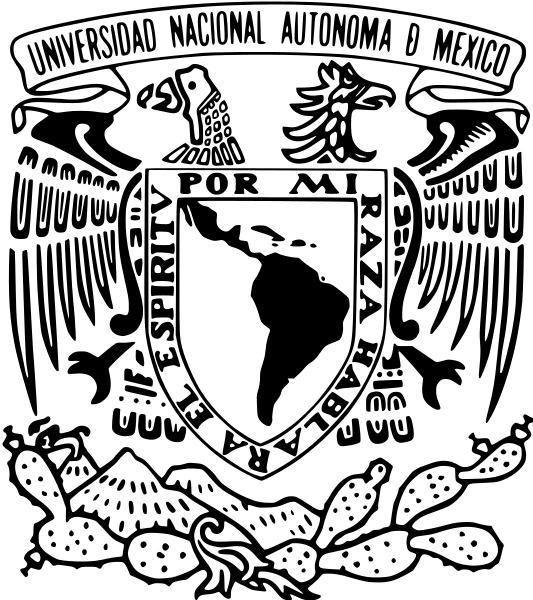
\includegraphics[width=0.24\textwidth]{../unam_logo.png} \hspace{1.5cm}
  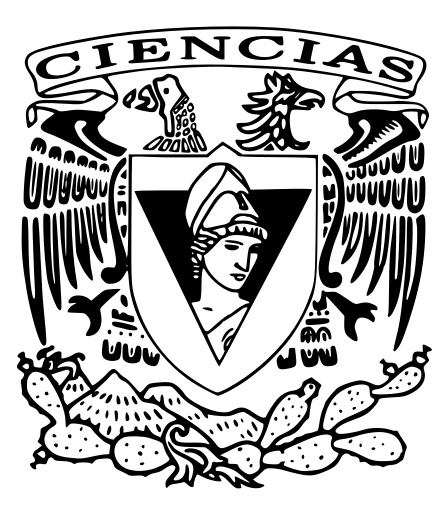
\includegraphics[width=0.25\textwidth]{../fc_logo.png} \\[1cm]
  \textbf{\Large UNIVERSIDAD NACIONAL AUTÓNOMA}\\[3mm]
  \textbf{\Large DE MÉXICO} \\[6mm]
  \textit{\Large Facultad de Ciencias}

  \vfill

  %---------------TÍTULO----------------->
  \linea
  \vfill \vspace{1cm}
  \textbf{\Large Compiladores}\\[1.1cm]
  \textbf{\Large Eliminación de Recursividad Izquierda,\\[0.2cm] Notación EBNF y Conjunto First}\\[0.9cm]
  \linea \\
  \vfill
  \vspace{0.7cm}
  %Title of the Research
  \textbf{\Large  Tarea 3}\\[6mm]
  %<<<<<<<<<<<<<<<<<<<<<<<<<<<<<<<<<<<<<<<<<<<

  %Team
  \vfill
  \textit{\small Presenta:}\\
  \textbf{\large  \textbf{Ramírez Juárez María Fernanda} - 321204747}\\[3mm]
  \textbf{\large  \textbf{Rojo Peña Manuel Ianluck} - 118005762}\\[3mm]

  %Profesor y Grupo
  \textit{\small Profesor:}\\
  \textbf{Pablo Martínez Yessica Janeth}\\[3mm]
  \textit{\small Ayudante:}\\
  \textbf{Rojas Fuentes Andrea}\\[3mm]
  \small Grupo: 7010, 2027-1\\[3mm]
  \vfill

  %Fecha or Date
  \textit{\small Fecha de entrega:}\\
         {\large 21 de septiembre, 2026}
         
\end{titlepage}


%%%%%%%%%%%%%%%%%%%%%%%%%%%%%%%%%%%%%%%%%%
\newpage
%%%%%%%%%%%%%%%%%%%%%%%%%%%%%%%%%%%%%%%%%%

\begin{enumerate}[label=\arabic*.]

\item Para cada una de las siguietnes gramáticas:

  \begin{enumerate}[label=\alph*.]
  \item Elimina la recursión por la izquierda.

  \item Escriba la gramática en notación EBNF.

  \item Dibuje los diagramas de sintaxis.

  \item Obtenga el conjunto First.
    
  \end{enumerate}

  \begin{itemize}
  \item Gramática 1:
    \[
    \begin{aligned}
      \nt{lexp} &\to \nt{atom} \mid \nt{list}\\
      \nt{atom} &\to \tk{num} \mid \tk{id}\\
      \nt{list} &\to \tk{(}\nt{lexp-seq}\tk{)}\\
      \nt{lexp-seq} &\to \nt{lexp} \nt{lexp-seq} \mid \nt{lexp}
    \end{aligned}
    \]

    \textbf{\large Eliminación por izquierda}:\\
    En esta gramática se observa que ninguna de sus reglas presenta recursividad por la izquierda, las
    producciones directas como:
    \[
    \begin{aligned}
      \nt{lexp} &\rightarrow \nt{atom} \mid \nt{list}\\
      \nt{atom} &\rightarrow \tk{num} \mid \tk{id}
    \end{aligned}
    \]
    
    son  derivaciones simples, La única regla recursiva es la de secuencias:
    \[
    \nt{lexp-seq} \rightarrow \nt{lexp}\tk{,} \nt{lexp-seq} \mid \nt{lexp}
    \]
    
    Dado que el no terminal \nt{lexp-seq} se llama a sí mismo en el extremo derecho de la producción, se trata
    de una recursividad por la derecha. Por lo tanto, la gramática ya cumple con la condición solicitada y no
    requiere aplicar eliminación por izquierda.\\

    \textbf{\large Notación EBNF}:\\
    La producción
    \[
    \nt{lexp-seq} \rightarrow \nt{lexp}\ \nt{lexp-seq} \mid \nt{lexp}
    \]
    
    genera simplemente una secuencia de una o más apariciones de \nt{lexp} concatenadas directamente
    (sin coma ni paréntesis entre ellas). En \textbf{EBNF}, la expresamos usando la cerradura de repetición.\\
    Las demás producciones se mantienen estructuralmente idénticas, ya que solo utilizan la alternancia
    directa.
    
    Por lo tanto, la Gramática 1 en \textbf{EBNF} queda así:

    \[
    \begin{aligned}
      \nt{lexp} &\rightarrow \nt{atom} \mid \nt{list}\\
      \nt{atom} &\rightarrow \tk{num} \mid \tk{id}\\
      \nt{list} &\rightarrow \tk{(}\ \nt{lexp-seq}\ \tk{)}\\
      \nt{lexp-seq} &\rightarrow \nt{lexp}\ \{\ \nt{lexp}\ \}
    \end{aligned}
    \]

    \newpage
    
    \textbf{\large Diagrama de sintaxis}:\\

    \begin{figure}[ht]
      \centering
      \includesvg[width=0.76\textwidth]{Gramatica1}
      \caption{Diagrama de sintaxis para la Gramática 1}
      \label{fig:diagrama_sintaxis}
    \end{figure}

    \newpage
    
    \textbf{\large Conjunto $\mathrm{FIRST}$}:\\

    \textbf{Paso 1. Terminales}
    
    \[
    \First{\nt{atom}} = \{\tk{num},\ \tk{id}\}
    \]
    
    \textbf{Paso 2. \nt{list}}\\
    Su producción empieza con el terminal \tk{(} por lo que no hay nada más que hacer, ya que el paréntesis no es
    anulable, el análisis se detiene en el primer símbolo, el resto del lado derecho es irrelevante.
    
    \[
    \First{\nt{list}} = \{\tk{(}\}
    \]
    
    \textbf{Paso 3. \nt{lexp}}\\
    Aquí sí hay dos alternativas y se unen los \textsc{First} de cada una:
    
    \[
    \begin{aligned}
      \First{\nt{lexp}}
      &= \First{\nt{atom}} \cup \First{\nt{list}} \\
      &= \{\tk{num},\ \tk{id}\} \cup \{\tk{(}\} \\
      &= \{\tk{num},\ \tk{id},\ \tk{(}\}
    \end{aligned}
    \]
    
    \textbf{Paso 4. \nt{lexp-seq}}\\
    La producción en EBNF es
    \[
    \nt{lexp-seq} \to \nt{lexp}\ \{\ \nt{lexp}\ \}
    \]
    Aquí ya no hay alternativas (\(\mid\)) que considerar: es una única secuencia formada por un \nt{lexp} obligatorio seguido de una repetición opcional de más \nt{lexp}. El símbolo con el que \emph{puede empezar} esta producción está determinado únicamente por el primer elemento obligatorio, es decir \nt{lexp}; la parte \(\{\ \nt{lexp}\ \}\) es opcional y por lo tanto no aporta símbolos iniciales adicionales (aunque casualmente en este caso serían los mismos, por ser el mismo no terminal repetido).

    \[
    \First{\nt{lexp-seq}} = \First{\nt{lexp}} = \{\tk{num},\ \tk{id},\ \tk{(}\}
    \]

    \textbf{Respuesta final}
    \[
    \begin{aligned}
      \First{\nt{lexp}}     &= \{\tk{num},\ \tk{id},\ \tk{(}\} \\
      \First{\nt{atom}}     &= \{\tk{num},\ \tk{id}\} \\
      \First{\nt{list}}     &= \{\tk{(}\} \\
      \First{\nt{lexp-seq}} &= \{\tk{num},\ \tk{id},\ \tk{(}\}
    \end{aligned}
    \]
    
  \item Gramática 2:
    \[
    \begin{aligned}
    \nt{S} &\to \nt{A}\ \nt{B}\\
    \nt{A} &\to \tk{begin } \nt{S } \tk{end } \nt{B } \tk{theend } \mid \eps\\
    \nt{B} &\to \tk{var} \nt{L} \tk{:} \tk{tipo} \mid \nt{B} \tk{fvar} \mid \eps\\
    \nt{L} &\to \nt{L}\tk{,} \tk{ id} \mid \tk{id}
    \end{aligned}
    \]

    \textbf{\large Eliminación por izquierda}:\\

    \begin{itemize}[leftmargin=*]
    \item \nt{S} / \nt{A}: \nt{A} $\rightarrow$ $\eps$ permite que \nt{S} derive directamente en \nt{B}, ninguna
      producción de \nt{B} empieza en \nt{S} ni en \nt{A}, así que no se propaga ninguna recursión hacia
      \nt{S} ni hacia \nt{A}.
      
    \item \nt{B}, por \nt{B} $to$ \nt{B} \tk{fvar} tenemos:
      \[
      \begin{aligned}
        \alpha_1 &= \tk{fvar},\\
        \beta_1 &= \tk{var}\ \nt{L}\ \tk{:}\ \tk{tipo},\\
        \beta_2 &= \eps
      \end{aligned}
      \]

      Cada $\beta$ se acompaña del nuevo no-terminal $\nt{B'}$, y $\beta_2 = \eps$ produce simplemente
      $\nt{B} \to \nt{B'}$:
      \[
      \begin{aligned}
        \nt{B}  &\to \tk{var}\ \nt{L}\ \tk{:}\ \tk{tipo}\ \nt{B'} \mid \nt{B'} \\
        \nt{B'} &\to \tk{fvar}\ \nt{B'} \mid \eps
      \end{aligned}
      \]
      
      Ese $\nt{B} \to \nt{B'}$ es una producción unitaria y la podemos dejar así para hacer la gramática más
      limpia:
      \[
      \nt{B} \to \tk{var}\ \nt{L}\ \tk{:}\ \tk{tipo}\ \nt{B'} \mid \tk{fvar}\ \nt{B'} \mid \eps
      \]
  
    \item \nt{L}, por \nt{L} $\to$ \nt{L} \tk{,} \tk{id} tenemos:
      \[
      \begin{aligned}
        \alpha &= \tk{,}\ \tk{id}\\
        \beta &= \tk{id}
      \end{aligned}
      \]

      Entonces:
      \[
      \begin{aligned}
        \nt{L}  &\to \tk{id}\ \nt{L'} \\
        \nt{L'} &\to \tk{,}\ \tk{id}\ \nt{L'} \mid \eps
      \end{aligned}
      \]
    \end{itemize}
    
    \textbf{Gramática Resultante:}
    \[
    \begin{aligned}
      \nt{S}  &\to \nt{A}\ \nt{B} \\
      \nt{A}  &\to \tk{begin}\ \nt{S}\ \tk{end}\ \nt{B}\ \tk{theend} \mid \eps \\
      \nt{B}  &\to \tk{var}\ \nt{L}\ \tk{:}\ \tk{tipo}\ \nt{B'} \mid \nt{B'} \\
      \nt{B'} &\to \tk{fvar}\ \nt{B'} \mid \eps \\
      \nt{L}  &\to \tk{id}\ \nt{L'} \\
      \nt{L'} &\to \tk{,}\ \tk{id}\ \nt{L'} \mid \eps
    \end{aligned}
    \]

    \medskip
    
    \textbf{\large Notación EBNF}:\\
    En vez de partir de las reglas ya transformadas (\nt{B'} y \nt{L'}), conviene derivar \textbf{EBNF} a partir
    del lenguaje que genera cada regla original, igual que se hizo con \nt{lexp-seq} en la Gramática 1.\\
    Usamos $[\ ]$ para lo opcional y $\{\ \}$ para lo repetible:

    \begin{itemize}[leftmargin=*]
    \item \nt{L} $\to$ \nt{L}\ \tk{,}\ \tk{id} $|mid$ \tk{id} genera una secuecnia d uno o más \tk{id} separados por comas, por lo que su cerradura de repetición es:
      \[
      \nt{L} \to \tk{id} \{\ \tk{,}\ \tk{id}\ \}
      \]

    \item \nt{B} $\to$ \tk{var} \nt{L} \tk{:} \tk{tipo} $\mid$ \nt{B} \tk{fvar} $\mid$ $\eps$ genera nada con cero o más \tk{fvar}, o bien, \tk{var} \nt{L} \tk{:} \tk{tipo} seguido de cero o más \tk{fvar}, es decir que la primera es opcional mientras que \tk{fvar} se repite:
      \[
      \nt{B} \to [\ \tk{var}\ \nt{L}\ \tk{:}\ \tk{tipo}\ ] \{\ \tk{fvar}\ \}
      \]
      
    \item \nt{A} $\to$ \tk{begin}\ \nt{S}\ \tk{end} \nt{B} \tk{theend} $\mid$ $\eps$ toda producción es opcional:
      \[
      \nt{A} \to [\ \tk{begin}\ \nt{S}\ \tk{end}\ \nt{B}\ \tk{theend}\ ]
      \]
      
    \item \nt{s} $\to$ \nt{A}\ \nt{B} no cambia, es un simple concatenación.
    \end{itemize}
    
    \textbf{Gramática Resultante:}
    \[
    \begin{aligned}
      \nt{S} &\to \nt{A}\ \nt{B} \\
      \nt{A} &\to [\ \tk{begin}\ \nt{S}\ \tk{end}\ \nt{B}\ \tk{theend}\ ] \\
      \nt{B} &\to [\ \tk{var}\ \nt{L}\ \tk{:}\ \tk{tipo}\ ]\ \{\ \tk{fvar}\ \} \\
      \nt{L} &\to \tk{id}\ \{\ \tk{,}\ \tk{id}\ \}
    \end{aligned}
    \]

    \newpage
    
    \textbf{\large Diagrama de sintaxis}:\\

    \begin{figure}[ht]
      \centering
      \includesvg[width=0.9\textwidth]{Gramatica2}
      \caption{Diagrama de sintaxis para la Gramática 2}
      \label{fig:diagrama_sintaxis}
    \end{figure}
        
    \newpage
    
    \textbf{\large Conjunto $\mathrm{FIRST}$}:\\

    \textbf{Paso 1. \nt{L}}\\
    La producción en EBNF es
    \[
    \nt{L} \to \tk{id}\ \{\ \tk{,}\ \tk{id}\ \}
    \]
    El símbolo obligatorio al inicio es \tk{id}, la parte $\{\ \tk{,}\ \tk{id}\ \}$ es opcional y no aporta nada nuevo al $\mathrm{FIRST}$. Como \tk{id} es un terminal, \nt{L} no es anulable, siempre debe generar al menos ese \tk{id}, entonces:

    \[
    \First{\nt{L}} = \{\tk{id}\}
    \]

    \textbf{Paso 2. \nt{B}}\\
    La producción es
    \[
    \nt{B} \to [\ \tk{var}\ \nt{L}\ \tk{:}\ \tk{tipo}\ ]\ \{\ \tk{fvar}\ \}
    \]
    
    Aquí hay dos partes opcionales, así que hay que unir los símbolos iniciales de cada una:
    \begin{itemize}[leftmargin=*]
    \item Si el bloque $[\ \tk{var}\ \nt{L}\ \tk{:}\ \tk{tipo}\ ]$ está presente, empieza con el terminal
      \tk{var}.
      
    \item Si el bloque está ausente, lo que sigue es $\{\ \tk{fvar}\ \}$, que empieza con \tk{fvar} si hay al
      menos una repetición, o puede no aportar nada si la repetición es cero.
    \end{itemize}
    
    Como ambos bloques opcionales pueden estar ausentes simultáneamente, \nt{B} sí es anulable ($\nt{B} \Rightarrow^* \eps$).
    \[
    \First{\nt{B}} = \{\tk{var}\} \cup \{\tk{fvar}\} = \{\tk{var},\ \tk{fvar}\}
    \]

    \textbf{Paso 3. \nt{A}}\\
    La producción es
    \[
    \nt{A} \to [\ \tk{begin}\ \nt{S}\ \tk{end}\ \nt{B}\ \tk{theend}\ ]
    \]
    
    Toda la producción es un único bloque opcional que, de estar presente, empieza con el terminal \tk{begin},
    no importa que dentro aparezca \nt{S} (que a su vez depende de \nt{A}), el primer símbolo. Si el bloque
    existe, siempre es el terminal \tk{begin}, así que no hay ninguna dependencia circular real que resolver
    aquí. Como el bloque completo es opcional, \nt{A} \textbf{es anulable} directamente.
    \[
    \First{\nt{A}} = \{\tk{begin}\}
    \]

    \textbf{Paso 4. \nt{S}}\\
    La producción es
    \[
    \nt{S} \to \nt{A}\ \nt{B}
    \]
    
    Es una concatenación simple, el $\mathrm{FIRST}$ de \nt{S} empieza con el $\mathrm{FIRST}$ de \nt{A}, pero
    como \nt{A} es anulable, también hay que agregar el $\mathrm{FIRST}$ de \nt{B}, el símbolo que le sigue:
    \[
    \begin{aligned}
      \First{\nt{S}}
      &= \First{\nt{A}} \cup \First{\nt{B}} \quad \text{(porque \nt{A} es anulable)}\\
      &= \{\tk{begin}\} \cup \{\tk{var},\ \tk{fvar}\} \\
      &= \{\tk{begin},\ \tk{var},\ \tk{fvar}\}
    \end{aligned}
    \]

    \textbf{Respuesta final}
    \[
    \begin{aligned}
      \First{\nt{S}} &= \{\tk{begin},\ \tk{var},\ \tk{fvar}\} \\
      \First{\nt{A}} &= \{\tk{begin}\} \\
      \First{\nt{B}} &= \{\tk{var},\ \tk{fvar}\} \\
      \First{\nt{L}} &= \{\tk{id}\}
    \end{aligned}
    \]
    
  \end{itemize}

  
%%%%%%%%%%%%%%%%%%%%%%%%%%%%%%%%%%%%%%%%%%
\newpage
%%%%%%%%%%%%%%%%%%%%%%%%%%%%%%%%%%%%%%%%%%

\item Construya el conjunto First de las siguientes gramáticas:

  \begin{enumerate}[label=\alph*.]
  \item
    
    \[
    \begin{aligned}
      \nt{declaracion} &\to \nt{tipo}\ \nt{var-list} \\
      \nt{tipo}        &\to \tk{int} \mid \tk{float} \\
      \nt{var-list}    &\to \tk{id}\ \tk{,}\ \nt{var-list} \mid \tk{id}
    \end{aligned}
    \]

    \textbf{Paso 1. Terminales}\\
    \nt{tipo} y \nt{var-list} tienen producciones que arrancan directamente con terminales, así que se resuelven
    sin depender de nadie.
    \[
    \begin{aligned}
      \First{\nt{tipo}}
      &= \First{\tk{int}} \cup \First{\tk{float}}
      = \{\tk{int},\ \tk{float}\} \\[2pt]
      \First{\nt{var-list}}
      &= \First{\tk{id}} \cup \First{\tk{id}}
      = \{\tk{id}\}
    \end{aligned}
    \]
    
    Las dos alternativas de \nt{var-list} empiezan con \tk{id}, así que la unión colapsa a un solo elemento.\\

    \textbf{Paso 2. \nt{declaracion}}\\
    Su única producción es $\nt{declaracion} \to \nt{tipo}\ \nt{var-list}$, el primer símbolo es \nt{tipo}, y
    $\eps \notin \First{\nt{tipo}}$ porque \nt{tipo} siempre produce \tk{int} o \tk{float}:
    \[
    \First{\nt{declaracion}} = \First{\nt{tipo}} = \{\tk{int},\ \tk{float}\}
    \]
    
    \textbf{Verificación por derivaciones.}\\
    Toda cadena del lenguaje se ve así:

    \[
    \begin{aligned}
      \nt{declaracion} &\Rightarrow \nt{tipo}\ \nt{var-list}
      \Rightarrow \tk{int}\ \nt{var-list}
      \Rightarrow \tk{int}\ \tk{id} \\
      \nt{declaracion} &\Rightarrow \nt{tipo}\ \nt{var-list}
      \Rightarrow \tk{float}\ \nt{var-list}
      \Rightarrow \tk{float}\ \tk{id}\ \tk{,}\ \tk{id}
    \end{aligned}
    \]

    El primer token es \tk{int} o \tk{float}, nunca \tk{id}, pues este aparece en la \emph{segunda} posición, y
    \textsc{First} no se entera de lo que pasa en la segunda posición.\\

    \textbf{Respuesta final}
    \[
    \begin{aligned}
      \First{\nt{declaracion}} &= \{\tk{int},\ \tk{float}\} \\
      \First{\nt{tipo}}        &= \{\tk{int},\ \tk{float}\} \\
      \First{\nt{var-list}}    &= \{\tk{id}\}
    \end{aligned}
    \]

    \newpage
    
  \item
    \[
    \begin{aligned}
      \nt{lexp}     &\to \nt{atom} \mid \nt{list} \\
      \nt{atom}     &\to \tk{num} \mid \tk{id} \\
      \nt{list}     &\to \tk{(}\ \nt{lexp-seq}\ \tk{)} \\
      \nt{lexp-seq} &\to \ \nt{lexp}\ \tk{,}\ \nt{lexp-seq} \mid \nt{lexp}
    \end{aligned}
    \]
    
    \textbf{Paso 1. Terminales}
    
    \[
    \First{\nt{atom}} = \{\tk{num},\ \tk{id}\}
    \]
    
    \textbf{Paso 2. \nt{list}}\\
    Su producción empieza con el terminal \tk{(}, no hay nada más que hacer, el resto del es irrelevante.
    
    \[
    \First{\nt{list}} = \{\tk{(}\}
    \]
    
    \textbf{Paso 3. \nt{lexp}}\\
    Aquí sí hay dos alternativas y se unen los \textsc{First} de cada una:
    
    \[
    \begin{aligned}
      \First{\nt{lexp}}
      &= \First{\nt{atom}} \cup \First{\nt{list}} \\
      &= \{\tk{num},\ \tk{id}\} \cup \{\tk{(}\} \\
      &= \{\tk{num},\ \tk{id},\ \tk{(}\}
    \end{aligned}
    \]
    
    \textbf{Paso 4. \nt{lexp-seq}}\\
    A diferencia del caso anterior, ahora ambas alternativas de
    \[
    \nt{lexp-seq} \to \nt{lexp}\ \tk{,}\ \nt{lexp-seq} \mid \nt{lexp}
    \]
    
    comienzan con el mismo no terminal \nt{lexp}, no hay ninguna alternativa que empiece directamente con un
    terminal, por lo tanto:
    \[
    \First{\nt{lexp-seq}} = \First{\nt{lexp}}
    \]
    
    Como \nt{lexp} no es anulable (no deriva $\eps$), no hace falta considerar lo que sigue después de \nt{lexp}
    en la primera alternativa; el cálculo se detiene ahí.
    
    \[
    \First{\nt{lexp-seq}} = \{\tk{num},\ \tk{id},\ \tk{(}\}
    \]
    
    \textbf{Respuesta final}
    \[
    \begin{aligned}
      \First{\nt{lexp}}     &= \{\tk{num},\ \tk{id},\ \tk{(}\} \\
      \First{\nt{atom}}     &= \{\tk{num},\ \tk{id}\} \\
      \First{\nt{list}}     &= \{\tk{(}\} \\
      \First{\nt{lexp-seq}} &= \{\tk{num},\ \tk{id},\ \tk{(}\}
    \end{aligned}
    \]
    
  \end{enumerate}
  
\end{enumerate}
\end{document}
